%% PI-AI-MM manuscript -- Nature Article format. Full rewrite of 2026-11-11 (previous version: ../review/nature_v1_2026-11-11/).
%% Order follows the Nature formatting guide: title, authors, bold referenced summary paragraph (<= 200 words), unheaded
%% introduction, main text with subheadings (<= 40 characters), references, Methods (with Data and Code availability),
%% end notes, Extended Data (1 figure, 7 tables). Main display items: Figs 1-4 and Table 1.
%% Page design: nature-style.tex. This file builds the clean reading copy; manuscript_submission.tex builds the same text
%% double-spaced with line numbers. tables/ and figures/ are copies of paper/tables and paper/figures
%% (refresh with: python refresh_from_package.py). Author-only items are marked \todo{...}.
\documentclass[11pt,a4paper]{article}
%% Shared page design for manuscript.tex and supplementary.tex (plain article class; Nature has no required LaTeX class
%% and takes a PDF at first submission). Two modes:
%%   reading mode (default)       : single-spaced, no line numbers -- a clean copy to read and circulate;
%%   submission mode              : double-spaced with line numbers, as the Nature formatting guide asks for a PDF submission.
%% Submission mode is switched on by defining \submissionmode before this file is read (see manuscript_submission.tex).

\usepackage[a4paper,left=22mm,right=22mm,top=24mm,bottom=26mm]{geometry}
\usepackage{iftex}
\ifPDFTeX                                   % pdfLaTeX (Overleaf default)
  \usepackage[T1]{fontenc}
  \usepackage{newtxtext,newtxmath}          % Times-like text and matching mathematics
  \usepackage[scaled=0.9]{helvet}           % Helvetica-like sans serif for title, headings, captions and tables
\else                                       % XeLaTeX / LuaLaTeX / tectonic
  \usepackage{newtxtext,newtxmath}
  \setsansfont{texgyreheros}[Extension=.otf,UprightFont=*-regular,BoldFont=*-bold,ItalicFont=*-italic,BoldItalicFont=*-bolditalic,Scale=0.9]
\fi
\usepackage{graphicx}
\usepackage{xcolor}
\usepackage{amsmath}
\usepackage{booktabs,tabularx,array}
\usepackage{float}
\usepackage{setspace}
\usepackage{url}
\usepackage[super,comma,sort&compress]{natbib}   % Nature: superscript reference numbers
\usepackage{titlesec}
\usepackage{caption}
\usepackage[hidelinks]{hyperref}

\bibliographystyle{sn-nature}
\providecommand{\bibcommenthead}{}          % written by sn-nature.bst; defined by the Springer class only
\renewcommand{\bibnumfmt}[1]{#1.}           % Nature reference list: "1." not "[1]"
\setlength{\bibsep}{2pt}
\renewcommand{\bibfont}{\small}

%% Headings: bold sans serif, unnumbered, close to the text they introduce.
\titleformat{\section}{\sffamily\bfseries\large\raggedright}{}{0pt}{}
\titlespacing*{\section}{0pt}{16pt plus 2pt minus 2pt}{4pt}
\titleformat{\subsection}{\sffamily\bfseries\normalsize\raggedright}{}{0pt}{}
\titlespacing*{\subsection}{0pt}{10pt plus 2pt minus 1pt}{2pt}
\newcommand{\bmhead}[1]{\subsection*{#1}}

%% Captions in Nature style: "Fig. 1 | Title. Text" and "Table 1 | Title", small sans serif, full width.
\DeclareCaptionLabelSeparator{bar}{\ \textbar\ }
\captionsetup{font={footnotesize,sf},labelfont=bf,labelsep=bar,justification=justified,singlelinecheck=false,skip=6pt}
\captionsetup[table]{position=top,textfont=bf,skip=4pt}
\renewcommand{\figurename}{Fig.}

%% One font for every table (the table files call \tablefont).
\newcommand{\tablefont}{\sffamily\fontsize{7.5}{9.5}\selectfont}
\renewcommand{\arraystretch}{1.1}

%% Floats: allow large figures and tables at the top of a page without pushing them to the end.
\renewcommand{\topfraction}{0.9}
\renewcommand{\bottomfraction}{0.6}
\renewcommand{\textfraction}{0.08}
\renewcommand{\floatpagefraction}{0.75}
\setlength{\textfloatsep}{14pt plus 2pt minus 2pt}
\floatplacement{table}{t}
\floatplacement{figure}{t}

\setlength{\parindent}{1.2em}
\setlength{\parskip}{0pt}
\emergencystretch=2em                       % no line may stick out into the margin
\frenchspacing
\raggedbottom

\ifdefined\submissionmode
  \usepackage{lineno}
  \renewcommand{\linenumberfont}{\normalfont\scriptsize\sffamily\color{black!55}}
  \setlength{\linenumbersep}{8pt}
  \AtBeginDocument{\doublespacing\linenumbers}
\fi

\newcommand{\todo}[1]{\textcolor{red}{[TODO: #1]}}
\newcommand{\muB}{\ensuremath{\mu_\mathrm{B}}}
\newcommand{\Tc}{\ensuremath{T_\mathrm{C}}}
\newcommand{\mcell}{\ensuremath{m_\mathrm{cell}}}
\newcommand{\mfu}{\ensuremath{m_\mathrm{fu}}}


\begin{document}
\pagestyle{plain}

\begin{flushleft}
{\sffamily\bfseries\fontsize{19}{23}\selectfont Reliability beyond accuracy in machine learning of magnetic materials\par}
\vspace{12pt}
{\sffamily\large Mujahidul Islam$^{1\,\ast}$ and Gayan P.~Hettiarachchi$^{1}$\par}
\vspace{6pt}
{\sffamily\footnotesize $^{1}$Digital Business and Innovation, Tokyo International University, 4-42-31 Higashi-Ikebukuro, Tokyo 170-0013, Japan.
$^{\ast}$e-mail: \href{mailto:mujahidmahfuz@gmail.com}{mujahidmahfuz@gmail.com}\par}
\end{flushleft}
\vspace{6pt}

%% Summary paragraph: bold, fully referenced, at most 200 words, few numbers and abbreviations, "Here we show".
{\bfseries\noindent Magnetic materials underpin electric motors, generators and data storage, and machine learning is widely used to search for new ones\cite{gutfleisch2011magnetic,coey2010magnetism}. Models trained on computed and literature-mined databases predict magnetic ordering and the Curie temperature from chemical composition, and are usually judged by their accuracy on held-out data\cite{nelson2019curie,long2021ferro,merker2022classifiers,itani2025nemad}. Such accuracy does not establish that added physical descriptors carry information, that stated uncertainties can be trusted or that predictions hold for unfamiliar chemistry, and these properties are rarely tested together\cite{meredig2018extrapolation,tran2020uq,kapoor2023leakage}. Here we show, with one curated dataset and one set of models, that they have to be measured separately. Descriptors from density functional theory gave no detectable gain over composition for ordering or the Curie temperature, and a small gain for the computed magnetic moment mostly reflected cell size. Prediction intervals were calibrated on average but under-covered the highest predictions, antiferromagnets and ferrimagnets unless the method was chosen with care. Ordering labels from computation and from experiment agreed no better than chance. On an audited external benchmark, error grew with chemical distance from the training data. Models intended for materials discovery should report descriptor gains, calibration and transfer alongside accuracy, because the candidates of interest lie far from the training data.\par}
\vspace{8pt}

%% ===================================================================================================================
%% Introduction (Nature Articles carry no heading here)

Three kinds of resource have made it possible to train machine-learning models of magnetism: high-throughput density functional theory (DFT) databases\cite{jain2013materials,saal2013oqmd,choudhary2020jarvis,curtarolo2012aflow}, databases mined from the literature\cite{kelly2025curie,court2020phase,itani2025nemad} and curated collections of magnetic structures\cite{gallego2016magndata}. Models that use only the chemical composition report errors of 56--69~K for the Curie temperature \Tc{} and accuracies of 78--91\% for magnetic ordering\cite{nelson2019curie,long2021ferro,belot2023curie,merker2022classifiers,itani2025nemad,abediorang2026curie}. Graph networks that read the crystal structure\cite{merker2022classifiers,choudhary2021alignn} and high-throughput DFT workflows\cite{horton2019ordering,frey2020oxides} offer other routes. These figures come from random or stratified splits of a single dataset (Supplementary Table~9). None of the studies that we examined tested on data grouped by chemistry or drawn from another label source, and in the one cross-dataset test that we found the \Tc{} error rose from 69 to 90~K\cite{belot2023curie}.

Accuracy on such splits is necessary, but work elsewhere in materials informatics shows that it is not sufficient. Random splits overstate the ability to extrapolate\cite{meredig2018extrapolation,xiong2020forwardcv,li2023critical,li2024mdhit,omee2024ood}. Accuracy on a proxy target need not carry over to the task of interest\cite{bartel2020stability}. Uncertainty estimates need their own validation\cite{tran2020uq,varivoda2023uq,palmer2022calibration}, and leakage between training and test data inflates reported performance\cite{kapoor2023leakage,dunn2020matbench}. Methods exist for distribution shift\cite{koh2021wilds,tibshirani2019covariate} and for abstaining from uncertain predictions\cite{geifman2017selective}, and active learning depends on uncertainty that can be used\cite{lookman2019active}. For magnetic materials, however, no single study has measured descriptor gains, calibration and transfer on the same data and the same models, with resampling at the level at which the records are dependent.

We made these measurements for three targets: magnetic ordering, \Tc{} and the magnetic moment computed by DFT. We asked whether DFT descriptors add information beyond composition, whether uncertainties are calibrated overall and within subgroups, and whether predictions transfer to unfamiliar chemistry and to labels from another source. The answers differ from question to question, and none follows from the accuracy of the model. Several errors that we made and corrected in our own earlier analyses (Methods) show how easily each question is answered wrongly.

%% ===================================================================================================================
\section*{Curated data and baselines}\label{sec:dataset}

We merged nine files from seven providers into one schema that records the source of every row (507,828 rows; Methods): Materials Project\cite{jain2013materials}, OQMD\cite{saal2013oqmd}, JARVIS-DFT\cite{choudhary2020jarvis}, two NEMAD releases\cite{itani2025nemad}, the ChemDataExtractor Curie and N\'eel database\cite{kelly2025curie}, MAGNDATA\cite{gallego2016magndata} and two experimental literature compilations. Written curation rules, which only remove rows, defined each target (Table~\ref{tab:table1_dataset}). Two removals were large. Five rules removed superconducting, ferroelectric and N\'eel temperatures and out-of-range values that had been recorded as Curie temperatures, which reduced the \Tc{} target from 34,322 to 29,740 records. All 15,493 JARVIS ordering labels were set aside, because every one read `ferromagnetic': the value was a default written by our data collector and not an assignment. The moment target is the total magnetic moment of the DFT cell at 0~K (\mcell{}); it is not an experimental saturation magnetization. Because \mcell{} grows with the number of atoms in the cell, we also analysed the moment per formula unit (\mfu{}).

The \Tc{} labels remain noisy after curation. In a screen of 200 randomly drawn records, judged from the title of the source paper, 11.0\% (95\% interval 7.4--16.1\%) were flagged as likely to be wrong; 12 of these 22 records came from the text-mined source, which supplied 61 of the 200. A further 16\% of the titles concerned a different compound, which a title alone cannot resolve, so the share of doubtful labels lies between 11\% and 27\% (Supplementary Table~5). Repeated records of one formula differ by a median standard deviation of 4.2~K, but for 13\% of such formulas the spread exceeds 100~K.

Predictors form three nested tiers. Tier~1 holds 65 descriptors computed from the composition alone. Tier~2 adds 8 descriptors of the oxidation states. Tier~3 adds 24 non-magnetic DFT properties of the most stable computed polymorph of each formula, such as the formation energy, band gap, symmetry, volume, density and elastic and dielectric constants (Methods), and is available for 28,512 materials. We kept the magnetic outputs of DFT out of Tier~3, because they are the source of the moment labels and of part of the ordering labels. Every split keeps all records of one reduced formula together.

\begin{table}
\caption{Prediction targets of the curated analysis dataset}
\label{tab:table1_dataset}
\tablefont
\begin{tabularx}{\textwidth}{@{}>{\raggedright\arraybackslash}Xlrrlr@{}}
\toprule
\textbf{Target} & \textbf{Unit} & \textbf{Records} & \textbf{Formulas} & \textbf{Train / validation / test} & \textbf{Matched records} \\
\midrule
Magnetic ordering (FM/AFM/FiM/NM) & class & 79,125 & 70,293 & 55,249/11,974/11,902 & 6,061 \\
Curie temperature & K & 29,740 & 14,145 & 20,508/4,691/4,541 & 4,602 \\
DFT total magnetic moment, per cell ($m_\mathrm{cell}$) & $\mu_\mathrm{B}$/cell & 87,513 & 77,402 & 61,254/13,130/13,129 & 10,852 \\
Mass magnetization (secondary) & emu/g & 4,317 & 3,218 & 3,021/648/648 & -- \\
Volume magnetization (secondary) & A/m & 779 & 454 & 535/124/120 & -- \\
Anisotropy constant $K_1$ (secondary) & J/m$^3$ & 1,847 & 1,182 & 1,296/280/271 & -- \\
\bottomrule
\end{tabularx}
\par\vspace{4pt}\raggedright\noindent Analysis dataset v1.4 (frozen); formula-grouped 70/15/15 splits. Matched records = materials with complete Tier 3 descriptors, used at every tier. Ordering classes: FM 34,098, NM 31,673, FiM 7,161, AFM 6,193. The DFT moment is the Materials Project/JARVIS total moment of the computed cell at 0 K (not an experimental saturation magnetization); the moment per formula unit ($m_\mathrm{fu}$ = $m_\mathrm{cell}\times$ atoms per formula unit / atoms in the cell, 10,821 matched rows) is analysed alongside. Tier 1 = 65 composition descriptors; Tier 2 = Tier 1 + 8 oxidation-state descriptors; Tier 3 = Tier 2 + 24 non-magnetic DFT descriptors (97).
\end{table}


Within the training distribution, composition alone was accurate. For ordering, XGBoost\cite{chen2016xgboost} reached a macro-averaged F1 score (macro-F1) of 0.727 (0.711--0.744), compared with 0.469 for multinomial logistic regression and 0.151 for the majority class. For \Tc{}, gradient boosting\cite{ke2017lightgbm,pedregosa2011sklearn} reached a mean absolute error (MAE) of 76.2~K (69.9--82.5~K) and a coefficient of determination $R^2$ of 0.78, compared with 147.2~K for ridge regression and 218.8~K for the training mean. For \mcell{}, gradient boosting reached 2.58~\muB{} per cell ($R^2$ 0.70). Compounds that are trivially non-magnetic do not carry the ordering score: over ten splits, restricting the test set to compounds that contain an element capable of magnetism lowered macro-F1 only from 0.692 to 0.681. The weak classes are antiferromagnets and ferrimagnets, with recalls near 0.55 and 0.49 (Supplementary Table~7).

%% ===================================================================================================================
\section*{Computed descriptors add little}\label{sec:rq1}

To test whether DFT descriptors add information, we compared the tiers on matched populations: the materials with complete Tier~3 descriptors, used with identical rows, splits, hyperparameter grids and metrics at every tier, over ten prespecified splits (Fig.~\ref{fig:rq1}, Extended Data Table~\ref{tab:table2_physics_descriptors}). We call a difference stable only if two intervals exclude zero, one that accounts for refitting\cite{nadeau2003inference} and one from a bootstrap over formulas, and if at least seven of the ten splits agree in sign. The nine contrasts between Tier~1 and Tier~3 (three targets by three algorithms) form the primary family and are Holm-corrected\cite{holm1979simple}.

For ordering and \Tc{}, no algorithm showed a stable effect of Tier~2 or Tier~3, and every primary adjusted $P$ value was 1.0. For \Tc{} the Tier~3 point estimates were losses: $-14.3$~K ($-42.5$ to $+13.9$) for gradient boosting, $-8.2$~K ($-48.3$ to $+32.0$) for XGBoost and $-14.4$~K ($-33.5$ to $+4.8$) for ridge regression with clipped inputs. This design detects only large effects, of 27--56~K for \Tc{} and 0.04--0.09 in macro-F1 for ordering, and the intervals leave room for \Tc{} gains of up to 5--32~K. We therefore report no detectable gain; we do not claim that a gain is absent. The matched \Tc{} population is also much harder than the full one (Tier~1 MAE 203~K, compared with 76~K), so the result applies to materials that have a full DFT record.

For \mcell{}, Tier~3 gave gains that were stable but small: $+0.079$~\muB{} per cell ($+0.030$ to $+0.127$) for gradient boosting and $+0.062$ ($+0.023$ to $+0.101$) for XGBoost, or 2--3\% of the MAE (adjusted $P=0.046$). A single number, the count of sites in the DFT cell, recovered about 70\% of the gradient-boosting gain when it was added to Tier~2, and what Tier~3 added beyond it was not resolved ($+0.024$; $-0.003$ to $+0.050$). The moment per formula unit behaved in the same way. Its gains were stable for all three algorithms ($+0.031$~\muB{} per formula unit for gradient boosting; $+0.014$ to $+0.048$), but beyond the site count they were not resolved for the two tree models, whereas ridge regression kept a stable $+0.030$ (Supplementary Table~8). Dividing the moment by the number of sites removes the cell size directly; a gain of 2.9\% of the MAE for gradient boosting, 2.8\% for XGBoost and 6.0\% for ridge regression then remained, and earlier analyses traced it mainly to other outputs of the same DFT calculation (Methods). The moment gain is therefore real but small, and for the per-cell and per-formula-unit targets it is mostly an effect of cell size.

\begin{figure}[t]
\centering
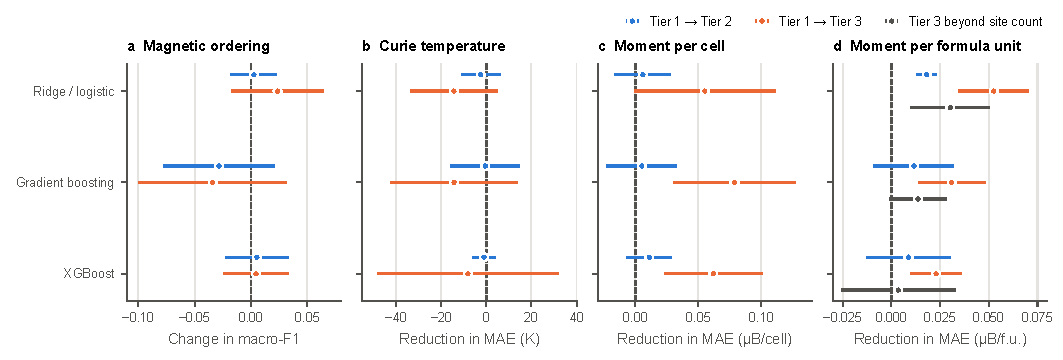
\includegraphics[width=\textwidth]{figures/fig1_physics_descriptors.pdf}
\caption{\textbf{Non-magnetic DFT descriptors add little beyond composition.} Change in test performance from Tier~1 (composition) to Tier~2 (oxidation states) and to Tier~3 (non-magnetic DFT descriptors) on identical matched materials. Points are means over ten prespecified formula-grouped splits and bars are 95\% intervals that account for refitting (Nadeau--Bengio); positive values are improvements. \textbf{a}, Macro-F1 for magnetic ordering. \textbf{b}, MAE for the Curie temperature; ridge regression uses clipped inputs. \textbf{c}, MAE for the DFT moment per cell. \textbf{d}, MAE for the DFT moment per formula unit, with the effect of Tier~3 beyond a single site-count descriptor. XGBoost values in \textbf{b} and \textbf{c} are means of eight realizations; those in \textbf{a} and \textbf{d} come from one.}\label{fig:rq1}
\end{figure}

A null result may reflect the choice of descriptors, because Tier~3 contains no magnetic quantities. For \Tc{}, where the magnetic outputs of DFT cannot leak the label, we therefore added three further kinds of physics to the matched population (Extended Data Table~\ref{tab:table3_magnetic_physics}): ten descriptors of the magnetic sublattice computed from the crystal structure, including the metal--anion--metal angles that govern superexchange; four magnetic outputs of DFT; and a fixed 64-dimensional crystal embedding from the pretrained interatomic potential CHGNet\cite{deng2023chgnet}. None improved on composition alone. Against Tier~1 the estimates ranged from $-10.8$ to $+9.5$~K, and every interval included zero. Relative to Tier~3, the embedding gave $+19.2$~K for XGBoost, which was stable in a single realization, and the magnetic outputs gave a borderline $+19.6$~K for gradient boosting. Both roughly recover the loss incurred at Tier~3, and neither exceeds Tier~1.

Feature attribution did not reveal this. TreeSHAP\cite{lundberg2017shap,lundberg2020treeshap} assigned 40\% (ordering) and 36\% (\Tc{}) of the mean absolute attribution of the Tier~3 XGBoost models to DFT descriptors that did not improve accuracy. Correlated composition and DFT features can carry the same information, so attribution shows that a feature is used and not that it adds value.

%% ===================================================================================================================
\section*{Average coverage hides failures}\label{sec:rq2}

We next asked whether the uncertainties can be trusted. For regression we compared three conformal methods\cite{vovk2005algorithmic,lei2018distribution,angelopoulos2023gentle} at a nominal coverage of 90\%: split conformal prediction, which gives intervals of constant width; normalized conformal prediction, which scales the width by a learned difficulty model\cite{papadopoulos2011normalized}; and conformalized quantile regression\cite{romano2019cqr} (Fig.~\ref{fig:rq2}a,b, Extended Data Table~\ref{tab:table4_regression_intervals}). On average all three met the nominal coverage, as the theory guarantees: 89.3\%, 90.3\% and 89.4\% for \Tc{}, and 90.0--90.1\% for \mcell{}.

The methods differed within subgroups, which we defined without reference to the difficulty score of any method. In the top decile of predicted \Tc{}, the normalized method covered 87.4\%, the constant-width method 65.5\% and quantile regression 68.6\%. For text-mined labels the figures were 86.0\% compared with 78--79\%, and for the highest predicted third of \mcell{} they were 86.7\% compared with 72.3\% and 83.4\%. The normalized method came closest to nominal coverage in these cases, but it was not best everywhere (Supplementary Table~11). On labels taken from computational papers it covered 86.6\%, compared with 90.4\% for the constant-width method; on several chemical families and on the two experimental compilations the other two methods covered more (92--97\% compared with 89--92\%), because their intervals are wide everywhere. The normalized method was the most stable: across splits its \Tc{} coverage had a standard deviation of 2.5 points, compared with about 6 points for the other two. Records of one formula are dependent, so about 4,200 calibration rows act like only 250--340 independent ones (Supplementary Table~6).

Coverage was not protected against shift. In the decile farthest from the training chemistry it was 86.6--89.7\%, and calibrating the normalized method separately for each distance quartile raised its coverage there from 88.2\% to 90.3\%. When intervals were calibrated on the larger experimental compilation and tested on text-mined rows (one frozen split), \Tc{} coverage was 76.9\% for the constant-width method, 80.3\% for quantile regression and 85.1\% for the normalized method.

The ordering classifier was trained with balanced class weights, so its raw probabilities follow a uniform prior. Correcting them to the training prior\cite{saerens2002adjusting} worsened the expected calibration error from 0.064 to 0.090, and adding temperature scaling\cite{guo2017calibration} reduced it to 0.014 (Extended Data Table~\ref{tab:table5_ordering_calibration}). Marginal conformal prediction sets met the nominal coverage overall (89.8\%) by covering ferromagnets (96.2\%) and non-magnets (97.7\%) too often, and antiferromagnets (57.0\%) and ferrimagnets (54.3\%) too rarely (Fig.~\ref{fig:rq2}c). Class-conditional sets\cite{vovk2013conditional} covered 89.8--90.9\% of every class, at a mean set size of 1.61 classes compared with 1.39.

\begin{figure}[t]
\centering
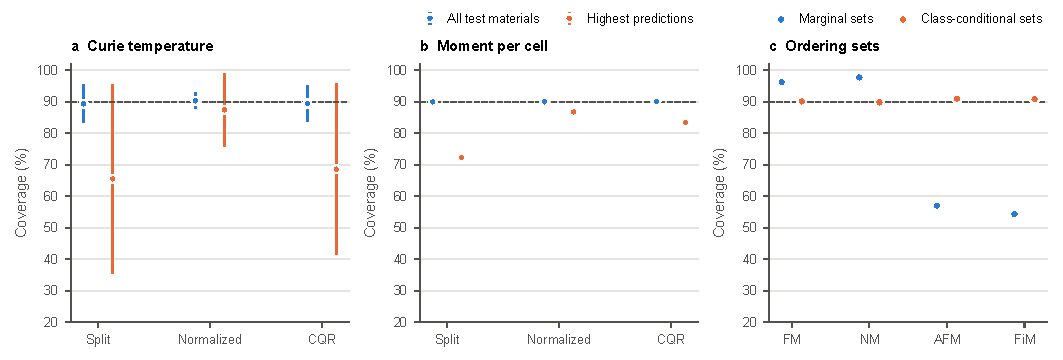
\includegraphics[width=\textwidth]{figures/fig2_uncertainty_calibration.pdf}
\caption{\textbf{Average coverage hides subgroup failures.} \textbf{a},\textbf{b}, Coverage of 90\% prediction intervals for the Curie temperature (\textbf{a}) and the DFT moment per cell (\textbf{b}), for all test materials and for the highest predictions (top decile in \textbf{a}, top third in \textbf{b}), under split, normalized and quantile (CQR) conformal prediction. Points are means over ten prespecified splits and bars are $\pm1$ s.d.\ across splits; in \textbf{b} the bars are smaller than the symbols. \textbf{c}, Mean coverage over the same splits of 90\% prediction sets for each ordering class (FM, ferromagnet; NM, non-magnet; AFM, antiferromagnet; FiM, ferrimagnet), for marginal and class-conditional sets. Dashed lines mark the nominal coverage.}\label{fig:rq2}
\end{figure}

%% ===================================================================================================================
\section*{Ordering labels depend on their source}\label{sec:provenance}

For 949 formulas, both Materials Project and an experimental source supply an ordering label. The two labels agreed for 28\% of these formulas, with Cohen's $\kappa=0.00$ ($-0.03$ to $0.03$), which is no better than chance. Of 508 antiferromagnets in the experimental sources, 336 (66\%) are ferromagnetic in Materials Project. This is what a high-throughput workflow produces when it starts from ferromagnetic configurations and enumerates antiferromagnetic orderings for only part of the database\cite{horton2019ordering}.

Models did not bridge this gap (Extended Data Table~\ref{tab:table7_generalization_internal}). A model trained on Materials Project labels and tested on experimental labels reached a balanced accuracy of 0.337 (0.273--0.396). This cannot be distinguished from models trained on permuted labels (median 0.342) and is far below the 0.769 of a model trained on experimental labels; its recall for antiferromagnets was 7\%. The test compositions were no farther from the training compositions than within Materials Project itself (median distance to the nearest training formula 0.081, compared with 0.077), so in this direction the failure lies in the definition of the labels and not in the chemistry. In the reverse direction the balanced accuracy was 0.384 (0.366--0.401), just above the 97.5th percentile of the permuted-label models (0.351) and far below the within-source value of 0.591. Here the chemistry differs as well (median distance 0.169, compared with 0.033 within the experimental sources), so the two causes cannot be separated. A pooled ordering score therefore measures agreement with a labelling convention as much as the ability to predict magnetic order.

%% ===================================================================================================================
\section*{Transfer to unfamiliar chemistry}\label{sec:rq3}

Within our data, holding out whole chemical systems (sets of elements) instead of formulas lowered the ordering macro-F1 from 0.712 to 0.684, a change of $-0.028$ ($-0.041$ to $-0.016$) that had the same sign in all ten paired splits and fell most heavily on ferrimagnets (Extended Data Table~\ref{tab:table7_generalization_internal}). The moment error rose slightly but not stably ($+0.073$~\muB{} per cell; $-0.009$ to $+0.154$), and the change in \Tc{} error was not resolved ($+2.7$~K; $-16.8$ to $+22.2$).

For an external test we used a public table of 2,500 experimental Curie temperatures that was curated for an independent study\cite{malaei_magnetic_data,abediorang2026curie}. We scored the Tier~1 XGBoost model for \Tc{} and its normalized conformal intervals on this table without retraining or tuning. An audit came first (Methods; Supplementary Table~1). When compositions were compared, and not formula strings, 1,998 records (80\%) were already in our repository, and 1,200 (48\%) carried a value within 0.5~K of one that we held. On those records the model scored $R^2$ 0.90, which measures recall of training labels and not prediction. After 105 records were excluded for stated reasons, 2,395 remained, of which 465 were compositions that the model had never seen.

On these 465 blind records, from 81 clusters of source papers, the MAE was 102.7~K (75.1--143.6~K) and $R^2$ was 0.69 (0.43--0.82), and the intervals covered 89.5\% (Fig.~\ref{fig:rq3}, Extended Data Table~\ref{tab:table6_external_benchmark}). Blind compositions in chemical systems that occur in the training data scored an MAE of 90.6~K and $R^2$ of 0.78. The 69 records in unseen chemical systems, from only 18 clusters, scored an MAE of 171.9~K (82.6--293.7~K) and $R^2$ of $-0.17$ ($-1.02$ to $0.64$). Performance in unseen systems is thus much weaker, with wide uncertainty. A rule that we fixed beforehand allows the statement `no skill beyond the mean' only if the upper limit of $R^2$ is at most 0.2, and that condition is not met; the upper limit is 0.21 even when chemical systems are the resampling unit (Supplementary Table~4). Skill in unseen chemical systems is therefore not established, and its absence is not established either.

\begin{figure}[t]
\centering
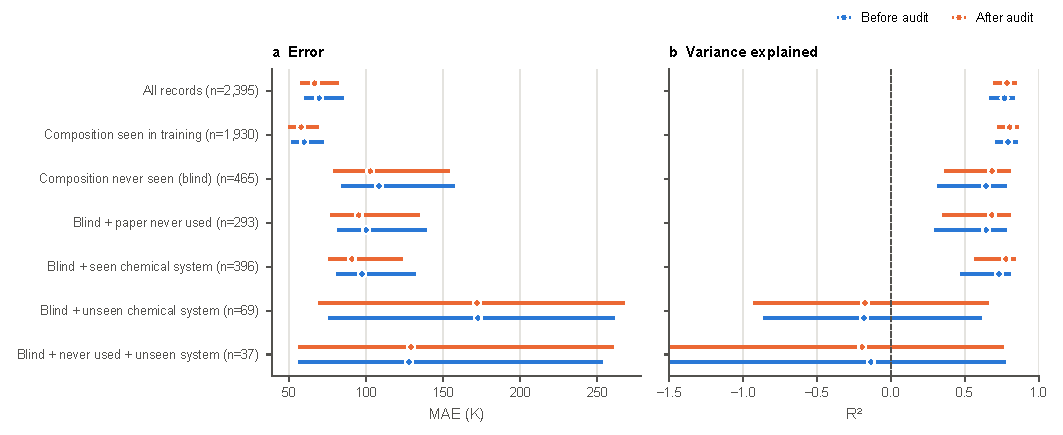
\includegraphics[width=\textwidth]{figures/fig3_external_benchmark.pdf}
\caption{\textbf{External benchmark of experimental Curie temperatures.} MAE (\textbf{a}) and $R^2$ (\textbf{b}) for nested novelty subsets of the external table, before and after the audit. Points are estimates and bars are 95\% percentile intervals from a bootstrap over clusters of source papers (10,000 resamples); bias-corrected intervals, which the text quotes, are in Extended Data Table~\ref{tab:table6_external_benchmark}. $n$ is the number of records after the audit, and lower limits of $R^2$ below $-1.5$ are cut off. `Blind' means that the composition never occurs in the training repository; `unseen system' means that its set of elements never occurs either.}\label{fig:rq3}
\end{figure}

Error followed a similarity measure that we fixed in advance, the composition distance to the nearest training formula. On the blind records, error rose with distance (Spearman's $\rho=0.28$; 0.10--0.49), and the MAE grew from 62~K in the closest quartile to 165~K in the farthest (Fig.~\ref{fig:distance}, Extended Data Fig.~\ref{fig:edscatter}). The normalized intervals widened, from 388 to 529~K, but not enough: coverage fell from 0.95 to 0.85 (Supplementary Table~3). Distance accounts for only part of the result for unseen systems, because blind records in seen systems at comparable distances kept an $R^2$ of 0.75.

\begin{figure}[t]
\centering
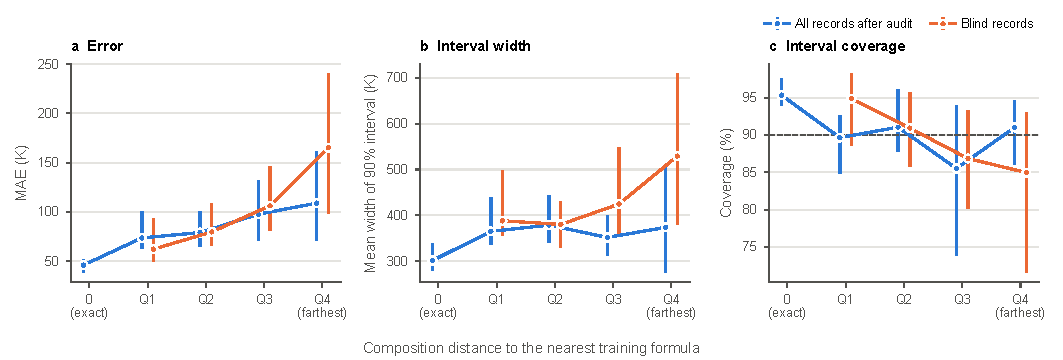
\includegraphics[width=\textwidth]{figures/fig4_error_vs_distance.pdf}
\caption{\textbf{Error grows and coverage falls with distance from the training chemistry.} External records binned by composition distance to the nearest training formula (bin 0, identical composition; Q1--Q4, quartiles of the non-zero distances), for all records after the audit and for the 465 blind records. \textbf{a}, MAE. \textbf{b}, Mean width of the 90\% interval. \textbf{c}, Coverage of the 90\% interval; the dashed line marks the nominal coverage. Bars are 95\% percentile intervals from a bootstrap over clusters of source papers.}\label{fig:distance}
\end{figure}

%% ===================================================================================================================
\section*{A first filter for screening}\label{sec:screening}

What do such predictions support in practice? On the 465 blind records, abstaining on the half of the compositions that lie farthest from the training data lowered the MAE from 103 to 71~K and brought coverage to 0.93 (Extended Data Table~\ref{tab:table8_screening}). Abstaining on the half with the widest intervals lowered the error by a similar amount (73~K) but left coverage at 0.88; the intervals of the two rules overlap, so we do not rank them. For a room-temperature screen (\Tc{} above 300~K; base rate 0.57), the point prediction had a recall of 0.94 and a precision of 0.77. Deciding only when the 90\% interval lay wholly above or wholly below 300~K settled 37\% of the records, with an accuracy of 92.5\%. The intervals are too wide to rank candidates within one family, but abstention and interval-based decisions make the model usable as a first filter.

%% ===================================================================================================================
\section*{Discussion}\label{sec:discussion}

The properties that we measured are related, but none can be inferred from another. Composition-only models were accurate, yet DFT descriptors gave no detectable gain while receiving more than a third of the attribution. The most accurate ordering model needed both prior correction and temperature scaling before its probabilities were calibrated, and its marginal prediction sets covered antiferromagnets and ferrimagnets little more than half the time. Intervals that were calibrated on average lost coverage with chemical distance and with a change of label source. A \Tc{} model with $R^2$ 0.78 inside the training distribution has no established skill in unseen chemical systems. An ordering model with macro-F1 0.73 transfers poorly between computed and experimental labels: at the level of permuted labels in one direction and barely above it in the other. Some of these outcomes were expected in principle, because marginal conformal guarantees do not extend to subgroups and balanced class weights distort probabilities. What we add is their size for magnetic materials, and evidence on which simple remedies work.

Why did DFT descriptors not help? We offer two explanations and have tested neither directly. First, the DFT values describe the lowest-energy computed polymorph of a formula, whereas a measured \Tc{} may belong to another structure, a doped sample or a film. The Tier~3 point estimates for \Tc{} were losses, which is consistent with such a noisy join. Second, composition already fixes much of what the scalar descriptors encode, and where a gain did appear it traced back largely to cell size. The null result is therefore narrow. It concerns descriptors joined by formula and used by tabular tree and linear models, together with one fixed embedding. It is not evidence against models that learn the coupling between structure and property end to end from the measured phase.

The study has limits. The external benchmark overlaps heavily with our sources, and the conclusion for unseen systems rests on 69 records from 18 clusters of papers. The label-noise screen was made from titles by an AI assistant, so its figures are estimates and not verified error rates. Formula-grouped splits are not perfectly disjoint: formulas written in two ways affect 0.6\% of the \Tc{} test rows and 1.3\% of the ordering test rows. The magnetic-physics test covers \Tc{} only, several comparisons rest on a single XGBoost realization, and we did not test end-to-end graph networks (Methods).

Several practices follow for evaluation. Descriptor sets should be compared on identical rows and repeated grouped splits, with an interval that accounts for refitting and a simple control for size. Coverage should be reported for subgroups that are defined independently of the uncertainty method. Novelty should be defined by composition and chemical system, and the values of an external test set should be checked against the training labels. Resampling should follow the dependence between records. Data collectors should be audited for default values, and labels for agreement across sources. For deployment, our results favour normalized or class-conditional conformal prediction, abstention far from the training data and recalibration when the label source changes. In discovery the candidates are unfamiliar by definition. A model for discovery should therefore be judged by how it behaves away from its training data and by whether its uncertainty supports a decision, and not by accuracy within the training distribution alone.

%% ===================================================================================================================
%% References. One list, numbered in order of first appearance; the Methods-only references are the last ones.
{\singlespacing
\bibliography{references}
}

%% ===================================================================================================================
\section*{Methods}\label{sec:methods}

\subsection*{Data collection and harmonization}
The sources were Materials Project\cite{jain2013materials} (100,000 entries); OQMD\cite{saal2013oqmd,kirklin2015oqmd}, obtained through jarvis-tools; JARVIS-DFT\cite{choudhary2020jarvis} (entries with a moment above 0.05~\muB{}); NEMAD\cite{itani2025nemad}; the ChemDataExtractor Curie and N\'eel database of Kelly and Cole\cite{kelly2025curie}; MAGNDATA\cite{gallego2016magndata,gallego2016magndata2}; and two experimental literature compilations of magnetic and anisotropy properties, whose origin is undocumented (Data availability). All sources were mapped to one schema of 25 columns. Each property kept its value, unit and measurement temperature, and each row kept the name of its source file. Records were deduplicated on material name and DOI together, so independent measurements of one composition were kept (507,828 rows). Formulas were made canonical with pymatgen\cite{ong2013pymatgen}. We set aside 1,940 records whose `formula' was not chemical, such as trade names and generic templates like ABO$_3$.

\subsection*{Descriptors}
Tier~1 (65 descriptors) holds composition statistics in the spirit of Magpie\cite{ward2016magpie}: element flags and fractions; fractions of transition-metal, rare-earth, actinide and magnetic elements; $s$, $p$, $d$ and $f$ fractions and counts of unpaired, $d$ and $f$ electrons; the valence-electron concentration; means and variances of radius, electronegativity, mass, melting temperature, period and group; and size mismatch and entropies. Tier~2 adds eight oxidation-state statistics from the charge-balancing routine of pymatgen. Tier~3 adds 24 non-magnetic DFT properties, joined by reduced formula from the most stable polymorph: formation energy, energy above the convex hull, band gap and band edges, Fermi level, space group, crystal system, point group, volume and density, elastic moduli, dielectric constants, refractive index and the maximum piezoelectric coefficient. Materials Project was the primary source; JARVIS supplied elastic and dielectric tensors where its coverage was denser, and AFLOW\cite{curtarolo2012aflow} supplied thermal properties. Seven properties were excluded by design: the magnetic flag, the number of magnetic sites, the magnetic species, the total magnetization, the magnetization per volume and the DFT ordering, which are close to the labels, and the elastic tensor, which is not a scalar. Four finite values that overflow single precision were set to missing.

\subsection*{Magnetic-physics test}
This test covers \Tc{} only. Crystal structures were retrieved for the same Materials Project entries (4,849 structures). Magnetic ions are the elements of curation rule C1 below, and bridging anions are O, S, Se, Te, N, P, As, F, Cl, Br and I. Ten sublattice descriptors were computed with pymatgen: the fraction and number density of magnetic sites; the shortest and the mean nearest metal--metal (M--M) distance; the number of M neighbours within 1.15 times the nearest M--M distance; the mean nearest metal--anion (M--X) distance and the M coordination (X within 1.2 times the nearest distance); the mean M--X--M angle around each anion over its bonded M neighbours, including periodic images; and the fractions of those angles in the ranges 150--180$^\circ$ and 80--100$^\circ$. The magnetic outputs of DFT were the moment per atom, the fraction of magnetic sites, the magnetization per volume and the magnetic flag. The CHGNet embedding is the 64-dimensional pooled crystal feature of the pretrained model (chgnet 0.4.2), used without further training\cite{deng2023chgnet}. XGBoost results in this test come from one realization.

\subsection*{Targets and curation}
For ordering, 116 raw labels were mapped to ferromagnetic (FM), antiferromagnetic (AFM), ferrimagnetic (FiM) and non-magnetic (NM). Hedged labels such as `ferromagnetic-like' and distinct states such as spin glasses and superparamagnets were excluded. Compensated ferrimagnets were kept as FiM. All JARVIS rows were set aside because their label was a constant written by the collector.

Curie temperatures were converted to kelvin. Placeholder zeros from one source and 54 encoded values were removed. Five rules then removed records: C1, formulas without an element capable of magnetism; C2, single elements that are not ferromagnets; C3, values below 1~K; C4, values above 1,400~K, which exceeds the highest known ferromagnetic \Tc{}, that of Co at about 1,388~K\cite{coey2010magnetism}; and C5, formulas labelled only AFM in every source. These rules are screens with known false positives; C1, for example, removes the ferromagnet YTiO$_3$. A sensitivity target without C5 gave the same baselines. The rules were written after the analyses of an earlier version of the dataset had been seen and before any model was fitted to the curated target.

For the title-based screen we drew a random sample of 200 curated records, stratified by source and by \Tc{} tercile (seed 20261110); the three sources supplied 61, 34 and 105 records, in proportion to their shares of the target. From the Crossref title, the compound and the value, and without reading the paper, each record was classified as a magnetic Curie transition, another kind of transition, an implausible value, a computational source, a paper about a different compound, a film or nanoscale sample, or unclear. The plan for this screen listed fewer categories; the categories `computational source', `implausible value' and `different compound' were added during classification. The `different compound' category (16.0\%) is not counted as wrong, because the title of a paper need not name every compound that it reports, which is why we give the range of 11--27\%. The classification was made by the AI assistant (see Use of large language models) \todo{and checked by the authors on N records with M disagreements: complete after the spot check}. The label of every record is released so that it can be checked.

The moment \mcell{} is the total moment of the computed cell at 0~K from Materials Project or JARVIS. For the 4,849 Materials Project entries whose records we retrieved, 99\% have energies in the mixed GGA and GGA+U scheme and 1\% in r$^2$SCAN alone, and the recorded orderings are 55\% FM, 27\% unknown, 8\% FiM, 6\% AFM and 4\% NM; most entries were computed from ferromagnetic initial configurations\cite{horton2019ordering}. The moment per formula unit is \mfu{} = \mcell{} $\times$ (atoms per formula unit)/(atoms in the cell), with the atom count of the same calculation (10,821 rows). We kept \mcell{} as the primary moment target because it is the quantity that the databases report and the one for which the comparisons were configured in advance. Mass and volume magnetization and the anisotropy constant $K_1$ are secondary targets and are not analysed here.

\subsection*{Splits, models and selection}
Records were split 70/15/15 by reduced formula, with a stratified assignment of groups that balances the sizes of the parts. Robustness analyses used ten splits with prespecified seeds ($20267000+i$), and the leave-chemical-system-out splits grouped records by their set of elements. The models were multinomial logistic or ridge regression with median imputation and standardization, histogram gradient boosting\cite{pedregosa2011sklearn,ke2017lightgbm} and XGBoost\cite{chen2016xgboost}; classifiers used balanced class weights. Hyperparameters were chosen on the validation macro-F1 (classification) or root-mean-square error (regression); the model was then refitted on the training and validation data and scored once on the test set. The grids were $C\in\{0.1,1,10\}$ or $\alpha\in\{0.1,1,10,100\}$ for the linear models; 500 iterations, a learning rate in $\{0.05,0.1\}$ and leaf nodes in $\{31,127\}$ for gradient boosting; and 500 trees, a depth in $\{6,10\}$, a learning rate in $\{0.05,0.1\}$ and subsample and column fractions of 0.8 for XGBoost. On the full populations, histogram gradient boosting reached an ordering macro-F1 of 0.720 and XGBoost a \Tc{} MAE of 75.4~K.

XGBoost results depend on the number of threads, which acts like a random seed: between settings the mean prediction changes by about 25\% of the MAE. Tier results for \Tc{} and \mcell{} are therefore averaged over eight realizations that differ in thread count and seed. The XGBoost tier results for ordering and for \mfu{} come from one realization; gradient boosting, which does not depend on the thread count, gives the same conclusions. Ridge regression without clipping produced exploded Tier~3 predictions from a few non-physical inputs (an elastic-anisotropy ratio of order $10^{110}$), so the ridge results for \Tc{} use inputs clipped to the 1st and 99th percentiles of the training fold.

\subsection*{Statistics}
Tier differences were computed on identical test materials. For each contrast we report the mean over the ten splits and two 95\% intervals: a pooled bootstrap over formulas (1,000 resamples, with the same draws for both tiers), and the corrected resampled-$t$ interval of Nadeau and Bengio, whose variance is inflated by $1/J+n_\mathrm{test}/n_\mathrm{train}$ to allow for the overlap between the $J$ splits\cite{nadeau2003inference}. Tests are two-sided. A contrast is stable if both intervals exclude zero and at least seven of the ten splits agree in sign, and borderline if only one interval excludes zero. The nine contrasts between Tier~1 and Tier~3 (three targets by three algorithms) form the primary family and are Holm-corrected\cite{holm1979simple}; the ridge member for \Tc{} is the contrast without clipping, and using the clipped contrast gives an adjusted $P$ of 0.74 for it and leaves the other eight unchanged. All other contrasts are secondary and unadjusted. Practical margins were fixed before the corresponding analyses: 10~K for \Tc{}, 0.02 for macro-F1 and 0.10~\muB{} per cell. The minimum detectable effect is stated at 80\% power; for the contrast between Tier~1 and Tier~3 it was 39~K (gradient boosting), 56~K (XGBoost) and 27~K (clipped ridge regression) for \Tc{}, and 0.040--0.091 in macro-F1 for ordering. Unless stated otherwise, ranges in parentheses in the main text are 95\% intervals.

Further contrasts were as follows. For ordering, the change from Tier~1 to Tier~2 under gradient boosting ($-0.028$) was a borderline loss: the bootstrap interval excluded zero and the refit-aware interval did not. For \mfu{}, the Tier~3 gains were $+0.023$ for XGBoost and $+0.053$ for ridge regression; beyond the site count they were $+0.014$ ($-0.001$ to $+0.028$; positive in nine of ten splits) for gradient boosting, $+0.004$ ($-0.026$ to $+0.033$) for XGBoost and a stable $+0.030$ ($+0.010$ to $+0.051$) for ridge regression. The per-atom gains had intervals across splits of 1.5--4.4\% (gradient boosting), 1.6--3.9\% (XGBoost) and 5.1--6.8\% (ridge regression). Analyses that added one descriptor family at a time attributed the per-atom gain mainly to other outputs of the same DFT calculation that produced the moment, and less to the volume descriptors. TreeSHAP rankings were stable over ten splits for ordering and the moment (mean pairwise Spearman correlation 0.96--0.98) but less so for \Tc{} (mean 0.91--0.94, minimum 0.83), so for \Tc{} we make statements about descriptor families only.

\subsection*{Planning and deviations}
The tier comparisons on ten splits were configured before their models were fitted. The later analyses were planned in writing before they were run, and the plan with its log of deviations is released (\texttt{results/revision/PLAN.md}). Six planned analyses were dropped for run time before any of their results were seen: the magnetic-physics test for ordering and for the moment; a \Tc{} comparison restricted to records whose source reports the same space group as the computed polymorph, which would have tested the `noisy join' explanation; a matched leave-chemical-system-out comparison; averaging over seeds for the ordering XGBoost models; a rerun of the moment intervals with per-row output; and a refit for the ordering decomposition, whose quantities were taken from saved probabilities instead.

\subsection*{Uncertainty quantification}
For regression intervals, whole formulas (20\% of the training formulas) formed the calibration set, and models were refitted on the remaining 80\%. Split conformal prediction used absolute residuals. Normalized conformal prediction divided them by a difficulty model fitted to cross-fitted absolute residuals. Conformalized quantile regression used XGBoost models for the 5\% and 95\% quantiles. Subgroups for evaluation were defined without the difficulty score of any method; Supplementary Table~11 lists every subgroup that we evaluated for \Tc{}. The moment subgroups come from an earlier run of the same code and splits. The design effect is $1+(\bar m-1)\rho$, where $\rho$ is the within-formula intraclass correlation of the indicator that a calibration row exceeds its interval and $\bar m$ is the size-weighted number of records per formula. It was 12--17, which implies a standard deviation of coverage between splits of 1.6--1.9 points. This accounts for much of the variability of the normalized method (2.5 points) and for little of that of the other two (about 6 points). Distance-aware (Mondrian) conformal prediction calibrates separately within each quartile of calibration distance; its coverage overall was 89.5\%. Weighted conformal prediction used a logistic density ratio in $\log(1+d)$\cite{tibshirani2019covariate}; it changed nothing, because the calibration and test sets come from the same pool. The source-shift coverages come from the single frozen split.

For ordering, probabilities were corrected to the training prior\cite{saerens2002adjusting} and temperature-scaled on half of the calibration formulas. Marginal and class-conditional thresholds on $1-p_\mathrm{true}$ were set on the other half\cite{vovk2013conditional}; fitting both on the same half changed coverage by less than 0.3 points. The expected calibration error is reported for the top label and classwise\cite{kull2019dirichlet}, with 15 bins of equal width. The classwise error changed much less than the top-label error (0.035 raw, 0.049 after prior correction, 0.032 with temperature scaling), so temperature scaling repairs the confidence and not the per-class probabilities. On the frozen split, marginal sets calibrated on Materials Project labels covered 83.5\% of experimental labels.

\subsection*{Cross-provenance ordering}
For formulas labelled by both Materials Project and an experimental source, we compared the most frequent label of each provenance (Cohen's $\kappa$, bootstrap over formulas; the full cross-tabulation is in Supplementary Table~12). For transfer, NM was removed everywhere, because the experimental labels contain only five NM rows. Models were trained on one provenance, after removal of training formulas that occur in the target test set and with hyperparameters selected on the validation rows of the source, and were tested on the test rows of the target, on the frozen split. The values in the main text use raw probabilities. With probabilities corrected to the class prior of the target domain, estimated from its training partition, the balanced accuracies were 0.314 (0.247--0.381) from Materials Project to experimental labels and 0.400 (0.370--0.430) in the reverse direction. The null distribution came from 20 refits on permuted training labels; its 97.5th percentiles were 0.374 and 0.351. Our plan allowed the statement that ordering `does not transfer' only if the upper limit of the corrected balanced accuracy lay below the 97.5th percentile of the null. The condition fails narrowly in one direction (0.381 against 0.374) and clearly in the other, so we report the size of the drop and do not make that statement.

\subsection*{Leave-chemical-system-out test}
This test used fixed hyperparameters on ten random splits of the full populations, so its baselines (for example 99~K for \Tc{}) differ from those of the frozen split. The formula-grouped and system-grouped schemes test different materials, so the reported changes combine novelty with differences in the composition of the test sets.

\subsection*{External benchmark and audit}
The external table\cite{malaei_magnetic_data,abediorang2026curie} lists 2,500 ferromagnets with experimental \Tc{} and source DOIs. The audit checks A1--A8 (Supplementary Table~1) were written down before any record-level error was linked to an audit flag or to a distance. They were written after the subset-level results of an earlier analysis were known; that analysis defined novelty by formula string and failed to match DOIs that carried a URL prefix (see Errors found and corrected). Three amendments were logged, one of them (clusters defined by the first-listed DOI) after the first bootstrap run. The 105 excluded records comprised 60 computational labels, 18 malformed compositions and 35 values outside our target definition; some records fall under more than one reason.

Novelty is defined by composition identity and by normalized DOIs. Distance is the total-variation distance between vectors of element fractions, taken to the nearest of 23,757 training formulas. Clusters are records linked by any shared DOI (the prespecified unit), by first-listed DOIs or by chemical systems. Intervals are percentile intervals and bias-corrected and accelerated intervals from a cluster bootstrap (10,000 resamples); the text quotes the latter. Skill is also measured against a fixed predictor equal to the training mean (\Tc{} = 338~K); for the records in unseen systems it was $-0.17$ ($-0.77$ to $0.56$). Before analysing the corrected subsets we fixed the wording rule quoted in the main text. The rule, too, was written after the subset results of the earlier, flawed analysis were known. With chemical systems as the resampling unit, the upper limits are 0.21 for $R^2$ and 0.17 for the fixed-reference skill.

The screening analysis of the 465 blind records was added later and was planned in writing. It also gave the precision among the highest-ranked predictions for \Tc{} above 300~K: 1.00 for the top 25 and the top 50 records and 0.93 for the top 100, against a base rate of 0.57.

\subsection*{Errors found and corrected}
During the study we found and corrected the following errors in our own work: a default `ferromagnetic' label written by the collector on all JARVIS entries (16\% of an earlier ordering target); transitions other than Curie transitions in the \Tc{} column; per-atom moments divided by the atom count of a different cell (25.4\% of rows); an external `blind' test that compared formula strings (1,302 records claimed blind, 502 by composition); a DOI normalizer that missed the \url{https://doi.org/} prefix; and a Tier~2 gain for ordering on a single split that did not replicate. In later rounds of checking we corrected a stability rule that was described more loosely than it was implemented, a difficulty subgroup defined by the method under test, a three-class chance reference for a four-class predictor, counts of papers reported in place of resampling clusters, and a wrong citation for the text-mined database. Earlier results are kept unchanged, and each correction is recorded in a versioned register of claims.

\subsection*{Use of large language models}
The data pipeline, the analyses and the manuscript were developed with substantial assistance from a large language model (Claude, Anthropic), which wrote code, ran analyses, classified the records of the title-based screen and drafted text under the direction of the authors. The authors checked the analyses and take full responsibility for the content. \todo{authors to confirm the extent of their checks before submission}

\subsection*{Data availability}
The curated analysis dataset (versions 1.2--1.4), the frozen splits, the adjudications of the external benchmark, the labels of the title screen and all result files form the reproducibility package \todo{repository and DOI}. Redistribution follows the terms of each source (Supplementary Table~10). Derived values from Materials Project, OQMD, JARVIS-DFT, the Kelly--Cole database and the Zenodo release of NEMAD are released under CC~BY~4.0 with attribution. The AFLOW terms permit non-commercial use only, MAGNDATA has no public licence, and the origin of the two experimental compilations is undocumented. The external benchmark table has no licence and is not redistributed; a script retrieves the analysed version and checks its SHA-256 hash. \todo{Before deposit: replace MAGNDATA, compilation and AFLOW values by identifiers plus retrieval scripts (or obtain permission), and drop the external compound names and values from the three result files that contain them.}

\subsection*{Code availability}
All analysis code, configurations with fixed seeds, the builders of the tables and figures, and the tests are in the reproducibility package, released under the MIT licence \todo{repository URL}. XGBoost results reproduce exactly only at the same thread count.

\bmhead{Acknowledgements}
\todo{acknowledgements, or delete this section}

\bmhead{Funding}
\todo{state funding, or ``The authors received no specific funding for this work.''}

\bmhead{Author contributions}
\todo{confirm: M.I. conceived the study, curated the data, developed the methods and software, performed the analyses and wrote the first draft. G.P.H. supervised the work, contributed to the methods and revised the manuscript.}

\bmhead{Competing interests}
The authors declare no competing interests.

\bmhead{Additional information}
\textbf{Supplementary information} is available for this paper (Supplementary Tables~1--12 and reproducibility notes). \textbf{Correspondence and requests for materials} should be addressed to Mujahidul Islam.

%% ===================================================================================================================
%% Extended Data (online only; at most ten items). Counters restart so that items read "Extended Data Fig. 1", "Extended Data Table 1", ...
%% Each item is fixed in place ([H]) in the order of first citation, so nothing drifts.
\clearpage
\ifdefined\submissionmode\nolinenumbers\fi
\setcounter{figure}{0}
\setcounter{table}{0}
\renewcommand{\figurename}{Extended Data Fig.}
\renewcommand{\tablename}{Extended Data Table}
\renewcommand{\theHfigure}{ED\arabic{figure}}
\renewcommand{\theHtable}{ED\arabic{table}}
\floatplacement{table}{H}
\floatplacement{figure}{H}
\section*{Extended Data}

\begin{figure}
\centering
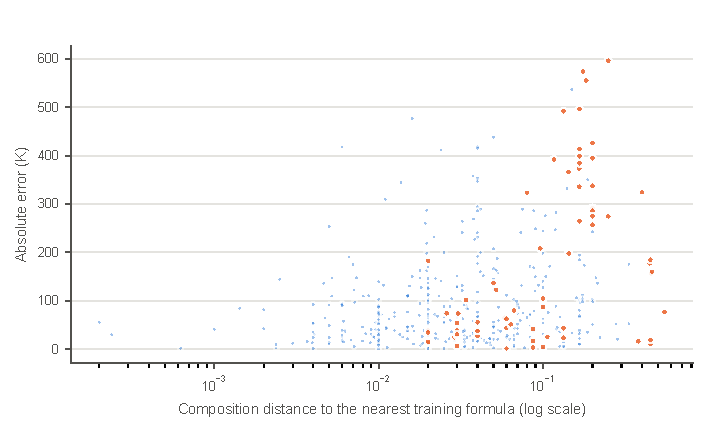
\includegraphics[width=120mm]{figures/figS1_blind_scatter.pdf}
\caption{\textbf{Error against chemical distance for every blind external record.} Absolute error of the predicted Curie temperature against the composition distance to the nearest training formula (logarithmic scale) for the 465 blind records of the external benchmark. Records in unseen chemical systems are highlighted.}\label{fig:edscatter}
\end{figure}

\vspace{10pt}
\begin{table}
\caption{Effect of oxidation-state (Tier 2) and DFT (Tier 3) descriptors on matched populations}
\label{tab:table2_physics_descriptors}
\tablefont
\begin{tabularx}{\textwidth}{@{}>{\raggedright\arraybackslash}Xlllrl@{}}
\toprule
\textbf{Algorithm} & \textbf{Tier 1$\rightarrow$2} & \textbf{Tier 1$\rightarrow$3} & \textbf{Verdict (1$\rightarrow$3)} & \textbf{Holm p} & \textbf{Tier 3 beyond site count} \\
\midrule
\multicolumn{6}{@{}l@{}}{\textit{Ordering, macro-F1}} \\
\quad Ridge / logistic & +0.003 [$-$0.018, +0.023] & +0.024 [$-$0.018, +0.065] & none & 1.000 & -- \\
\quad Gradient boosting & $-$0.028 [$-$0.078, +0.021] & $-$0.034 [$-$0.100, +0.032] & none & 1.000 & -- \\
\quad XGBoost & +0.005 [$-$0.023, +0.033] & +0.004 [$-$0.024, +0.033] & none & 1.000 & -- \\
\addlinespace
\multicolumn{6}{@{}l@{}}{\textit{Curie temperature, MAE (K)}} \\
\quad Ridge (clipped inputs) & $-$2.5 [$-$11.1, +6.2] & $-$14.4 [$-$33.5, +4.8] & none & -- & -- \\
\quad Gradient boosting & $-$0.4 [$-$15.7, +14.9] & $-$14.3 [$-$42.5, +13.9] & none & 1.000 & -- \\
\quad XGBoost & $-$1.0 [$-$6.0, +3.9] & $-$8.2 [$-$48.3, +32.0] & none & 1.000 & -- \\
\addlinespace
\multicolumn{6}{@{}l@{}}{\textit{Moment per cell, MAE ($\mu_\mathrm{B}$/cell)}} \\
\quad Ridge / logistic & +0.006 [$-$0.016, +0.028] & +0.055 [$-$0.001, +0.111] & none & 0.373 & -- \\
\quad Gradient boosting & +0.005 [$-$0.023, +0.033] & +0.079 [+0.030, +0.127] & stable gain & 0.046 & -- \\
\quad XGBoost & +0.011 [$-$0.007, +0.029] & +0.062 [+0.023, +0.101] & stable gain & 0.046 & -- \\
\addlinespace
\multicolumn{6}{@{}l@{}}{\textit{Moment per formula unit, MAE ($\mu_\mathrm{B}$/f.u.)}} \\
\quad Ridge / logistic & +0.018 [+0.013, +0.023] & +0.053 [+0.035, +0.070] & stable gain & -- & +0.030 [+0.010, +0.051] \\
\quad Gradient boosting & +0.012 [$-$0.009, +0.032] & +0.031 [+0.014, +0.048] & stable gain & -- & +0.014 [$-$0.001, +0.028] \\
\quad XGBoost & +0.009 [$-$0.013, +0.030] & +0.023 [+0.010, +0.036] & stable gain & -- & +0.004 [$-$0.026, +0.033] \\
\bottomrule
\end{tabularx}
\par\vspace{4pt}\raggedright\noindent Improvement = deeper tier minus Tier 1 performance, positive = better; identical matched rows, splits, grids and metrics at every tier; 10 prespecified formula-grouped splits. Intervals: Nadeau-Bengio corrected resampled-t 95\% (refit-aware). Stable = this interval AND the pooled formula-bootstrap interval exclude 0 AND at least 7 of 10 splits share the sign; borderline = only one of the two intervals excludes 0; none = no stable change. Holm p over the primary family (9 Tier 1$\rightarrow$3 contrasts: ordering, Curie, moment per cell x 3 algorithms). XGBoost = mean over 8 thread/seed realizations (Curie, moment per cell); single realization for ordering and the moment per formula unit. Curie Ridge uses train-fold 1st/99th-percentile clipping; unclipped Ridge is numerically unstable ($-$825 K) and is not interpretable. The Curie Ridge member of the Holm family is the unclipped contrast (adjusted p = 1.000); using the clipped contrast instead gives 0.740 for that contrast and leaves the other eight unchanged. The ordering gradient-boosting Tier 1$\rightarrow$2 change is a borderline loss (the bootstrap interval excludes 0, the refit-aware interval does not). Moment per formula unit: 10,821 rows; 'beyond site count' = Tier 3 vs Tier 2 + the number of sites in the DFT cell.
\end{table}

\clearpage
\begin{table}
\caption{Magnetic and structure-aware physics for the Curie temperature}
\label{tab:table3_magnetic_physics}
\tablefont
\begin{tabularx}{\textwidth}{@{}>{\raggedright\arraybackslash}Xrllll@{}}
\toprule
\textbf{Algorithm} & \textbf{MAE (K)} & \textbf{vs Tier 1} & \textbf{Verdict vs Tier 1} & \textbf{vs Tier 3} & \textbf{Verdict vs Tier 3} \\
\midrule
\multicolumn{6}{@{}l@{}}{\textit{Tier 1 + magnetic-sublattice geometry (10)}} \\
\quad Gradient boosting & 202.6 & +0.3 [$-$13.9, +14.5] & none & -- & -- \\
\quad XGBoost & 203.6 & +5.8 [$-$15.8, +27.4] & none & -- & -- \\
\addlinespace
\multicolumn{6}{@{}l@{}}{\textit{Tier 3 + magnetic-sublattice geometry}} \\
\quad Gradient boosting & 220.2 & -- & -- & $-$3.1 [$-$27.6, +21.4] & none \\
\quad XGBoost & 211.0 & -- & -- & +8.0 [$-$15.8, +31.9] & none \\
\addlinespace
\multicolumn{6}{@{}l@{}}{\textit{Tier 3 + DFT magnetic outputs (4)}} \\
\quad Gradient boosting & 197.6 & +5.3 [$-$29.9, +40.4] & none & +19.6 [$-$3.1, +42.3] & borderline gain \\
\quad XGBoost & 210.7 & $-$1.4 [$-$35.8, +33.0] & none & +8.3 [$-$27.5, +44.2] & none \\
\addlinespace
\multicolumn{6}{@{}l@{}}{\textit{Tier 3 + geometry + DFT magnetic outputs}} \\
\quad Gradient boosting & 205.6 & $-$2.8 [$-$39.1, +33.6] & none & +11.5 [$-$14.4, +37.4] & none \\
\quad XGBoost & 201.9 & +7.5 [$-$33.8, +48.8] & none & +17.2 [$-$9.5, +43.9] & borderline gain \\
\addlinespace
\multicolumn{6}{@{}l@{}}{\textit{Tier 3 + CHGNet crystal embedding (64)}} \\
\quad Gradient boosting & 213.7 & $-$10.8 [$-$22.5, +0.9] & none & +3.5 [$-$19.2, +26.2] & none \\
\quad XGBoost & 199.9 & +9.5 [$-$28.7, +47.7] & none & +19.2 [+0.4, +38.0] & stable gain \\
\bottomrule
\end{tabularx}
\par\vspace{4pt}\raggedright\noindent Matched Curie population (4,602 records), same 10 splits as Extended Data Table 1; MAE of Tier 1 / Tier 3: gradient boosting 202.9 / 217.1 K, XGBoost 209.3 / 219.1 K. Geometry: magnetic-ion site fraction and density, nearest and mean M-M distance, M-M connectivity, M-X distance and coordination, mean M-X-M angle and the fractions of angles in [150, 180] and [80, 100] degrees, from the Materials Project structure of the same entry. DFT magnetic outputs (moment per atom, magnetic-site fraction, magnetization per volume, magnetic flag) are not label leakage for experimental Curie temperatures. CHGNet = frozen 64-d crystal feature of the pretrained universal potential. Improvement in K, positive = better; Nadeau-Bengio 95\% intervals; verdict 'none' = no stable change; XGBoost single realization.
\end{table}

\vspace{10pt}
\begin{table}
\caption{Coverage of 90\% conformal prediction intervals, overall and in subgroups}
\label{tab:table4_regression_intervals}
\tablefont
\begin{tabularx}{\textwidth}{@{}>{\raggedright\arraybackslash}Xlllll@{}}
\toprule
\textbf{Method} & \textbf{All, mean (SD)} & \textbf{Mean width} & \textbf{High predictions} & \textbf{Second subgroup} & \textbf{Farthest distance decile} \\
\midrule
\multicolumn{6}{@{}l@{}}{\textit{Curie temperature}} \\
\quad Split conformal & 89.3 (6.0) & 569 K & top decile 65.5 & text-mined 78.2 & 86.6 \\
\quad Normalized conformal & 90.3 (2.5) & 451 K & top decile 87.4 & text-mined 86.0 & 88.2 \\
\quad CQR & 89.4 (5.8) & 519 K & top decile 68.6 & text-mined 79.3 & 89.7 \\
\addlinespace
\multicolumn{6}{@{}l@{}}{\textit{Moment per cell}} \\
\quad Split conformal & 90.0 (0.4) & 12.6 $\mu_\mathrm{B}$/cell & top third 72.3 & oxides 84.0 & -- \\
\quad Normalized conformal & 90.0 (0.5) & 11.7 $\mu_\mathrm{B}$/cell & top third 86.7 & oxides 91.0 & -- \\
\quad CQR & 90.1 (0.4) & 9.8 $\mu_\mathrm{B}$/cell & top third 83.4 & oxides 89.5 & -- \\
\bottomrule
\end{tabularx}
\par\vspace{4pt}\raggedright\noindent Nominal 90\%; 10 prespecified formula-grouped splits; calibration on 20\% of training formulas; coverage in \%. Subgroups are defined without any method's own difficulty score: top decile of the point prediction (Curie) or highest predicted third (moment), the text-mined label source (Curie) or oxides (moment), and the farthest decile of composition distance to the proper-training formulas. For comparison, on the decile defined by the normalized method's own difficulty scale (a circular definition used in an earlier analysis) coverage is 54/89/61\% for split/normalized/CQR (Curie).
\end{table}

\clearpage
\begin{table}
\caption{Calibration of magnetic-ordering probabilities and prediction sets}
\label{tab:table5_ordering_calibration}
\tablefont
\begin{tabularx}{\textwidth}{@{}>{\raggedright\arraybackslash}Xrrrrrrrr@{}}
\toprule
\textbf{Probabilities / sets} & \textbf{Top-label ECE} & \textbf{Classwise ECE} & \textbf{Coverage (\%)} & \textbf{FM} & \textbf{AFM} & \textbf{FiM} & \textbf{NM} & \textbf{Set size} \\
\midrule
raw (balanced-weight) probabilities & 0.064 & 0.035 & -- & -- & -- & -- & -- & -- \\
prior-corrected & 0.090 & 0.049 & -- & -- & -- & -- & -- & -- \\
prior-corrected + temperature & 0.014 & 0.032 & -- & -- & -- & -- & -- & -- \\
Class-conditional sets & -- & -- & 90.1 (0.6) & 90.1 & 90.9 & 90.8 & 89.8 & 1.61 \\
Marginal sets & -- & -- & 89.8 (0.9) & 96.2 & 57.0 & 54.3 & 97.7 & 1.39 \\
\bottomrule
\end{tabularx}
\par\vspace{4pt}\raggedright\noindent Mean over 10 prespecified splits (Tier 1 XGBoost, full ordering population); 15 equal-width bins. Sets at 90\% nominal on prior-corrected, temperature-scaled probabilities, with the temperature fitted on half of the calibration formulas and the conformal thresholds on the other half (re-using one calibration set gives the same coverage to within 0.3 points). Coverage = mean (SD).
\end{table}

\vspace{10pt}
\begin{table}
\caption{Generalization to unfamiliar chemical systems and to another label provenance}
\label{tab:table7_generalization_internal}
\tablefont
\begin{tabularx}{\textwidth}{@{}>{\raggedright\arraybackslash}Xlll>{\raggedright\arraybackslash}X@{}}
\toprule
\textbf{Target} & \textbf{Metric} & \textbf{Familiar $\rightarrow$ unfamiliar} & \textbf{Change [95\% CI]} & \textbf{Reference} \\
\midrule
\multicolumn{5}{@{}l@{}}{\textit{Leave chemical system out (10 paired splits)}} \\
\quad Ordering & macro-F1 & 0.712 $\rightarrow$ 0.684 & $-$0.028 [$-$0.041, $-$0.016] & 10/10 splits worse \\
\quad Curie temperature & MAE & 99.2 $\rightarrow$ 101.9 & +2.7 [$-$16.8, +22.2] & 5/10 splits worse \\
\quad Moment per cell & MAE & 2.591 $\rightarrow$ 2.663 & +0.073 [$-$0.009, +0.154] & 7/10 splits worse \\
\addlinespace
\multicolumn{5}{@{}l@{}}{\textit{Label agreement, MP vs experimental (949 shared formulas)}} \\
\quad Ordering & agreement / $\kappa$ & 0.28 / 0.00 & $\kappa$ [$-$0.03, 0.03] & $\kappa$ = 0: chance agreement \\
\addlinespace
\multicolumn{5}{@{}l@{}}{\textit{Label provenance: train MP $\rightarrow$ test experimental (FM/AFM/FiM)}} \\
\quad Ordering & balanced accuracy & 0.769 $\rightarrow$ 0.337 & 0.337 [0.273, 0.396] & shuffled-label null, 97.5th pct 0.374 \\
\addlinespace
\multicolumn{5}{@{}l@{}}{\textit{Label provenance: train experimental $\rightarrow$ test MP (FM/AFM/FiM)}} \\
\quad Ordering & balanced accuracy & 0.591 $\rightarrow$ 0.384 & 0.384 [0.366, 0.401] & shuffled-label null, 97.5th pct 0.351 \\
\bottomrule
\end{tabularx}
\par\vspace{4pt}\raggedright\noindent Leave chemical system out: the test sets differ between the two schemes (formula- vs chemical-system-grouped), so the change mixes novelty with test-set composition. Provenance: NM removed on both sides (the experimental labels contain 5 NM rows); training formulas present in the target test set removed; 'familiar' = the same model trained and tested within the target provenance; null = 20 refits with permuted training labels; formula-cluster bootstrap 95\% intervals.
\end{table}

\clearpage
\begin{table}
\caption{Independent experimental Curie benchmark by novelty subset}
\label{tab:table6_external_benchmark}
\tablefont
\begin{tabularx}{\textwidth}{@{}>{\raggedright\arraybackslash}Xrlllr@{}}
\toprule
\textbf{Subset} & \textbf{n (clusters)} & \textbf{MAE, K} & \textbf{R$^2$} & \textbf{Skill vs training mean} & \textbf{90\% coverage} \\
\midrule
All records & 2,395 (464) & 66.5 [57.2, 81.1] & 0.79 [0.69, 0.85] & 0.80 [0.70, 0.85] & 0.925 \\
Composition seen in training & 1,930 (440) & 57.7 [50.7, 70.4] & 0.80 [0.72, 0.86] & 0.83 [0.74, 0.87] & 0.933 \\
\quad seen, value not copied & 767 (208) & 84.5 [68.1, 110.2] & 0.70 [0.53, 0.80] & 0.71 [0.53, 0.81] & 0.890 \\
Composition never seen (blind) & 465 (81) & 102.7 [75.1, 143.6] & 0.69 [0.43, 0.82] & 0.70 [0.41, 0.84] & 0.895 \\
Blind + source paper never used & 293 (61) & 95.1 [73.1, 125.7] & 0.68 [0.43, 0.83] & 0.72 [0.50, 0.86] & 0.898 \\
Blind + seen chemical system & 396 (72) & 90.6 [71.8, 116.0] & 0.78 [0.67, 0.87] & 0.79 [0.66, 0.89] & 0.902 \\
Blind + unseen chemical system & 69 (18) & 171.9 [82.6, 293.7] & $-$0.17 [$-$1.02, 0.64] & $-$0.17 [$-$0.77, 0.56] & 0.855 \\
Blind + never used + unseen system & 37 (12) & 129.0 [61.8, 297.0] & $-$0.19 [$-$6.17, 0.70] & 0.04 [$-$1.03, 0.69] & 0.757 \\
\bottomrule
\end{tabularx}
\par\vspace{4pt}\raggedright\noindent Primary benchmark after the audit (2,395 of 2,500 records); seen/blind by composition identity. Clusters = source-paper components (records linked by any shared DOI), the resampling unit; 95\% BCa cluster-bootstrap intervals (10,000 resamples). Skill = 1 - MSE / MSE of a constant prediction equal to the training mean (338 K), a fixed reference across subsets. Results under first-DOI and chemical-system clustering are in Supplementary Table 4.
\end{table}

\vspace{10pt}
\begin{table}
\caption{What the predictions support in a screening setting (blind external compositions)}
\label{tab:table8_screening}
\tablefont
\begin{tabularx}{\textwidth}{@{}>{\raggedright\arraybackslash}Xrl@{}}
\toprule
\textbf{Use} & \textbf{n (papers)} & \textbf{Result} \\
\midrule
Abstain on composition distance, keep 100\% & 465 (81) & MAE 103 [78, 154] K; coverage 0.89 [0.83, 0.92] \\
Abstain on composition distance, keep 50\% & 238 (42) & MAE 71 [61, 97] K; coverage 0.93 [0.88, 0.96] \\
Abstain on interval width, keep 50\% & 233 (50) & MAE 73 [59, 109] K; coverage 0.88 [0.77, 0.92] \\
$T_\mathrm{C}$ > 300 K from the point prediction: accuracy & 465 (81) & 0.802 [0.717, 0.879] \\
\quad recall & 465 (81) & 0.936 [0.866, 0.973] \\
\quad precision & 465 (81) & 0.769 [0.667, 0.902] \\
Decide only when the 90\% interval excludes 300 K: share decided & 465 (81) & 0.374 [0.261, 0.598] \\
\quad accuracy of those decisions & 465 (81) & 0.925 [0.837, 0.982] \\
\bottomrule
\end{tabularx}
\par\vspace{4pt}\raggedright\noindent The 465 truly blind external records; base rate of $T_\mathrm{C}$ > 300 K = 0.57. Paper-cluster bootstrap 95\% intervals (10,000 resamples). Distance = composition (total-variation) distance to the nearest training formula; width = width of the normalized-conformal interval.
\end{table}


\end{document}
